\title{Questions workflow systeem\\ELGG plugin\\
\includegraphics[width=0.40\textwidth]{img/logo.png}
}
\author{
  Bart Jeukendrup\\
  bart@infty.io
}
\date{\today}

\documentclass[12pt]{article}
\usepackage{graphicx}

\begin{document}
\maketitle

\begin{abstract}
Dit document geeft een korte uitleg van het workflow systeem geïmplementeerd in de ELGG plugin Questions. Het workflow systeem geeft een organisatie de mogelijkheid om op een gefaseerde manier vragen te beantwoorden. Hierdoor kunnen verschillende afdelingen bijdragen aan een gezamelijk antwoord. 
\end{abstract}

\section{Het workflow systeem configureren}
Het workflowsysteem kan geactiveerd worden door een subsite beheerder via het subsite beheerscherm (https://deelsite.pleio.nl/admin/). Zorg allereerst dat de Questions plugin geactiveerd is (Plugins). Ga vervolgens naar instellingen, Questions. Het workflow systeem kan nu geactiveerd worden door bij workflow activeren op 'ja' te zetten. Daarnaast is het van belang om ook expert rollen in te schakelen.

\subsection{Fases configureren}
In het configuratiescherm wordt verder gevraagd om fases te definieren. Het workflowsysteem bevat minimaal $2$ fases. Per fase is het mogelijk om een maximale looptijd in te stellen. Bij overschrijding van deze looptijd kleurt de fase rood. Verder kan er een e-mailadres gekoppeld worden aan elke fase. Als een vraag in een bepaalde fase geplaatst wordt stuurt het systeem automatisch een e-mail naar dit adres. 

\subsection{Werktijden configureren}
Als laatste kunnen bij de plugin instellingen de werktijden ingesteld worden. Het systeem berekent op basis van deze werktijden de looptijd van een fase. Uren buiten werktijden tellen niet mee. 

\section{Expert rollen toewijzen}

\begin{figure}
  \centering
  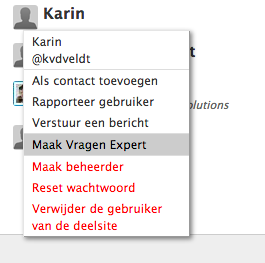
\includegraphics[width=0.25\textwidth]{img/add-expert.png}
  \caption{Expert rol toewijzen}
  \label{fig:expert}
\end{figure}

Alle personen met een expert rol krijgen automatisch toegang tot het workflow systeem (zie figuur \ref{fig:expert}). Expert rollen kunnen toegewezen worden aan personen door op het pijltje onder hun avatar te klikken, en te kiezen voor de optie 'maak vragen expert'. Nu heeft deze gebruiker toegang tot het workflow systeem. Het is aan te raden dit ook voor het eigen deelsite beheerders account te doen om toegang te krijgen tot het workflow systeem.

\section{Workflow gebruiken}

\begin{figure}
  \centering
  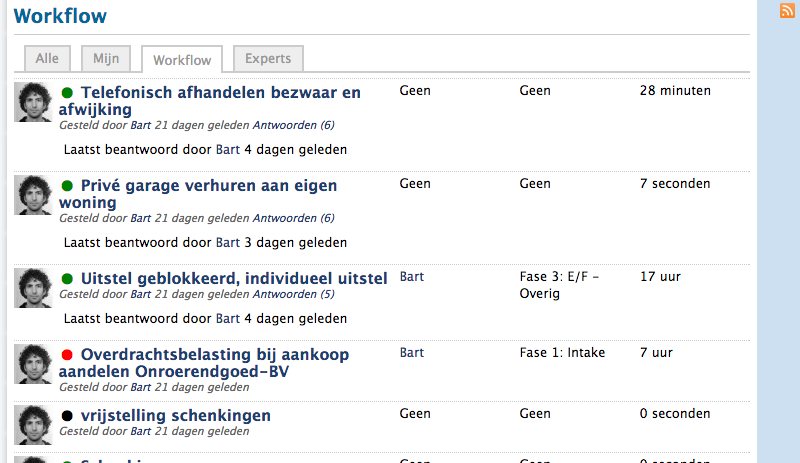
\includegraphics[width=0.75\textwidth]{img/workflow-overview.png}
  \caption{Het workflow dashboard}
  \label{fig:dashboard}
\end{figure}

Het workflowsysteem is nu bereikbaar via de voorkant (https://deelsite.pleio.nl/questions/). Door op het tabblad 'workflow' te klikken, verschijnt een overzicht van het workflowdashboard (zie figuur \ref{fig:dashboard}). Het dashboard kent per vraag drie kleuren. Wanneer een vraag in behandeling is kan de vraag groen of rood zijn. Groen wanneer de maximale fasetijd nog niet verstreken is, rood wanneer de maximale fasetijd wel verstreken is. Wanneer een vraag niet in behandeling is kan de vraag zwart of groen zijn. Zwart wanneer er een nieuwe reactie op de voorkant is gekomen, maar er nog geen keuze is gemaakt om de workflow te heropenen of gesloten te houden en groen wanneer alle reacties op de voorkant tot dan toe verwerkt zijn.

\section{Doorlopen van een workflowcyclus}
We geven nu een voorbeeldje van een complete workflowcyclus. Gebruiker plaatst eerst een vraag via de voorkant, bijvoorbeeld 'Telefonisch afhandelen bezwaar en afwijking'. In het workflowsysteem verschijnt de vraag automatisch ook. Aan de vraag is nog geen fase toegekend. De workflowmedewerker kan vervolgens een keuze maken: of de vraag wordt geopend, of de vraag blijft gesloten (zie figuur \ref{fig:question-detail}). Kiest de medewerker voor 'gesloten houden', dan kleurt de vraag groen en blijft de vraag de status groen behouden tot er nieuwe reacties op de vraag komen. Wanneer de vraag wordt geopend gaat de looptijd lopen en wordt de vraag automatisch in de eerste fase van het workflowsysteem geplaatst. De bal ligt nu bij de verantwoordelijke voor de eerste fase van het workflow systeem. Deze persoon formuleert een antwoord en kiest na het formuleren van het antwoord direct de vervolgfase. Zo kan de vraag meerdere fases doorlopen. De maximale looptijd van elke fase wordt iedere keer bijgehouden. Wanneer een vraag meerdere keren in dezelfde fase terecht komt, worden de looptijden bij elkaar opgeteld. Wanneer het workflowsysteem in de laatste fase geplaatst wordt krijgt de medewerker de mogelijkheid om de vraag ook op de voorkant te publiceren. Dat betekent dat het antwoord ook leesbaar is op de voorkant, dus de persoon die de vraag heeft gesteld. Door het plaatsen van de workflow in de laatste fase wordt de workflowcyclus automatisch gesloten.

\begin{figure}
  \centering
  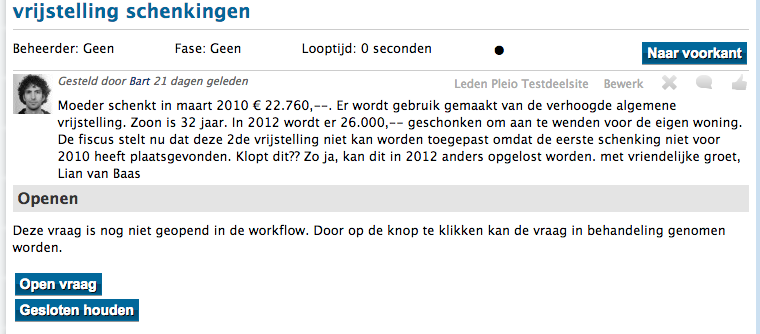
\includegraphics[width=0.75\textwidth]{img/detail-question.png}
  \caption{Vraag detail}
  \label{fig:question-detail}
\end{figure}

\section{Metadata per intern antwoord}
Op het moment dat een intern antwoord wordt opgeslagen, wordt de looptijd van het antwoord berekend (het verschil tussen het huidige moment en het einde van de vorige fase). Daarnaast wordt de fase waarin het antwoord is gegeven opgeslagen en of het antwoord ook op de voorkant is gepubliceerd. Daarnaat wordt opgeslagen of het workflowsysteem met het antwoord gesloten is.

\section{Verschillende workflow cycli}
Het is mogelijk om per vraag meerdere beantwoordingscycli te hebben. Een voorbeeld: Gebruiker plaatst de vraag 'Telefonisch afhandelen bezwaar en afwijking'. Vervolgens wordt de vraag in behandeling genomen en doorloopt achtereenvolgens drie fases. Uiteindelijk wordt een antwoord geplaatst op de voorkant en wordt de cyclus afgesloten. De gebruiker stelt vervolgens onder het antwoord een nieuwe vraag. De medewerker besluit om de workflow weer te openen. Het hele proces begint nu weer opnieuw. De resultaten van de verschillende cycli worden afzonderlijk gerapporteerd in de Business Intelligence component.

\section{Workflowsysteem en groepen}
Wanneer de questions plugin gebruikt wordt binnen groepen, kan het workflowsysteem per groep aan of uitgezet worden. Raadpleeg hiervoor de groep instellingen. Daarnaast kunnen experts per groep toegewezen worden.

\section{Business Intelligence}
Het workflowsysteem biedt de mogelijkheid om een CSV bestand te exporteren met alle gerealiseerde workflowcycli. Raadpleeg hiervoor de plugin instellingen van de deelsite. Onder het kopje Workflow systeem bevindt zich de knop 'Download CSV export'.
De CSV export bevat per vraag één of meerdere regels afhankelijk van het aantal cycli dat doorlopen is. Per cyclus is vermeld hoeveel seconden een vraag in een bepaalde fase staat. Daarnaast bevat iedere regel de vraag titel, de aanmaaktijd de huidige workflow status, het aantal antwoorden en het aantal interne antwoorden.

\end{document}